\chapter{HASIL DAN PEMBAHASAN}
\label{hasil-dan-pembahasan}
Bangunan yang dijadikan objek penelitian adalah \textit{climate chamber} DTNTF FT UGM. Dalam bab ini, akan dibahas mengenai hasil rancang bangun sistem kendali sesuai dengan langkah-langkah yang dijelaskan pada Bab IV dengan memvariasikan berbagai macam masukan, kemudian mengetahui keluarannya. Variasi masukan dan keluaran akan dimodelkan dengan model jaringan saraf tiruan untuk mendapatkan parameter-parameter model yang dapat mengendalikan sistem bangunan.

\section{Hasil Pengambilan Data Simulasi IES-VE}

\subsection{Kondisi \textit{Climate Chamber}}
\begin{figure}[!h]
	\centering
	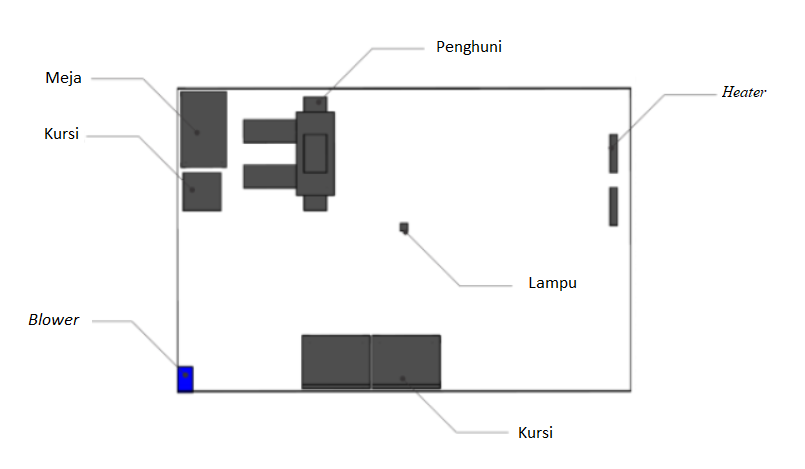
\includegraphics[width=1\textwidth]{figures/KondisiChamber}
	\caption{Posisi Komponen \textit{Climate Chamber}}
	\label{fig:5:KondisiChamber}
\end{figure}

\textit{Climate chamber} memiliki ukuran $3m \times 2m \times 3m$ ($p \times l \times t$). Komponen-komponen di dalam \textit{climate chamber} terdiri dari meja, kursi, \textit{blower}, penghuni, lampu, \textit{heater}, dan AC. 

\begin{figure}[h]
	\centering
	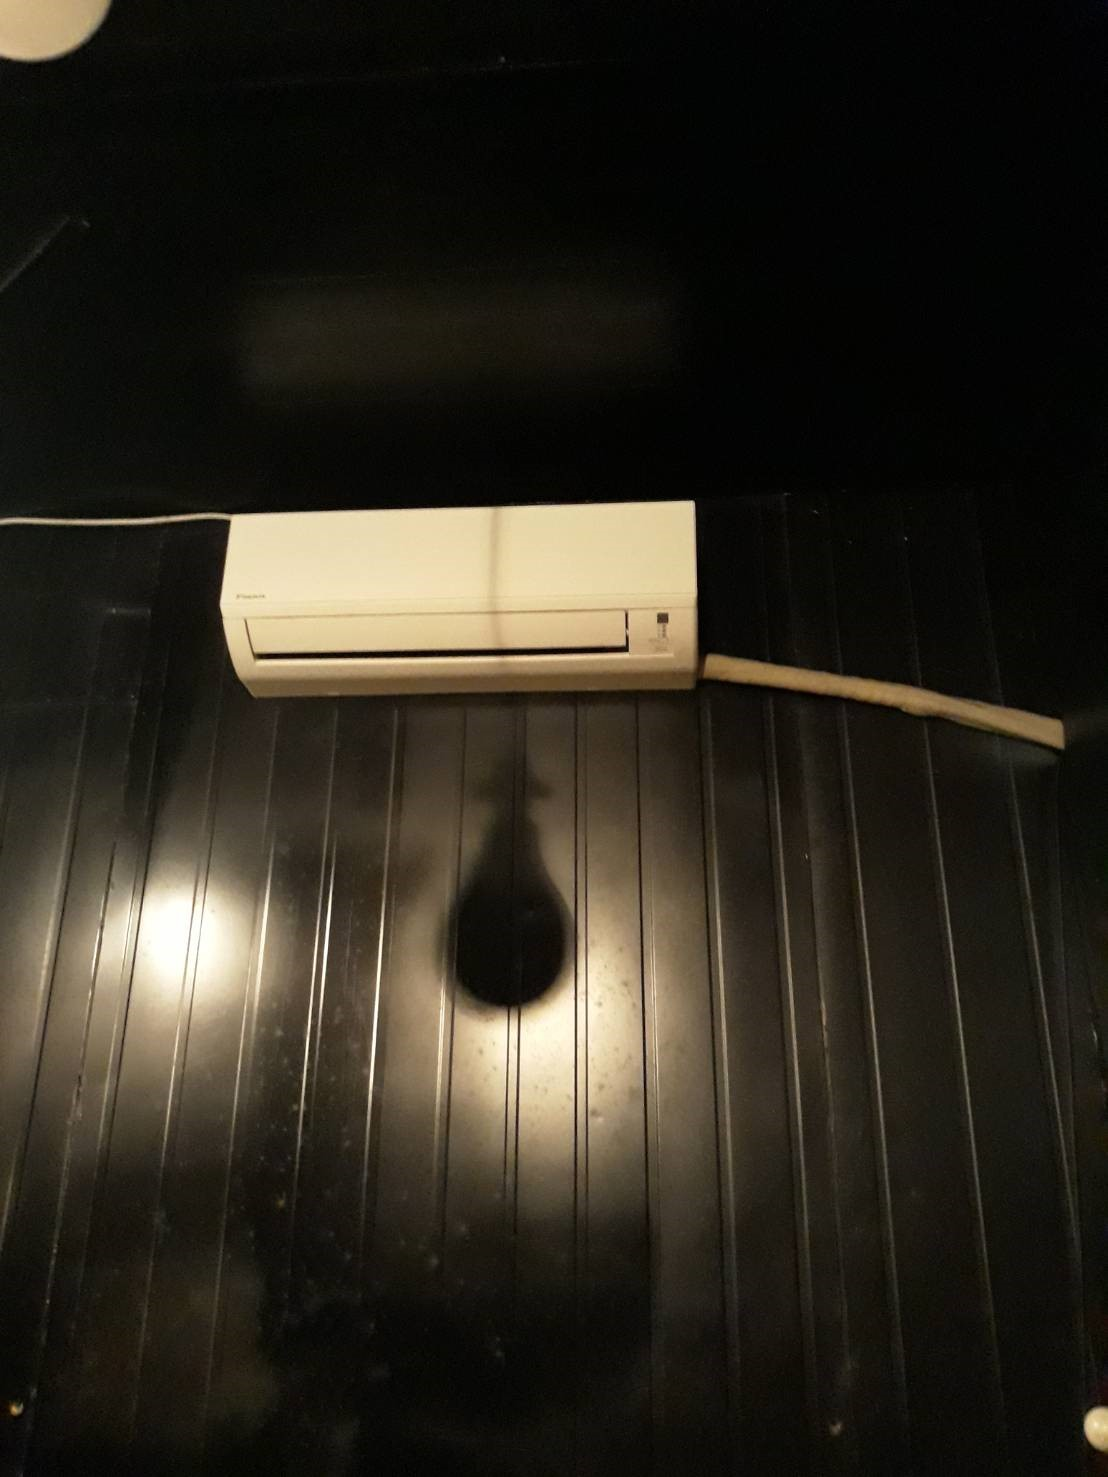
\includegraphics[width=0.8\textwidth]{figures/AC}
	\caption{Perangkat AC}
	\label{fig:5:AC}
\end{figure}

\begin{figure}[!h]
	\centering
	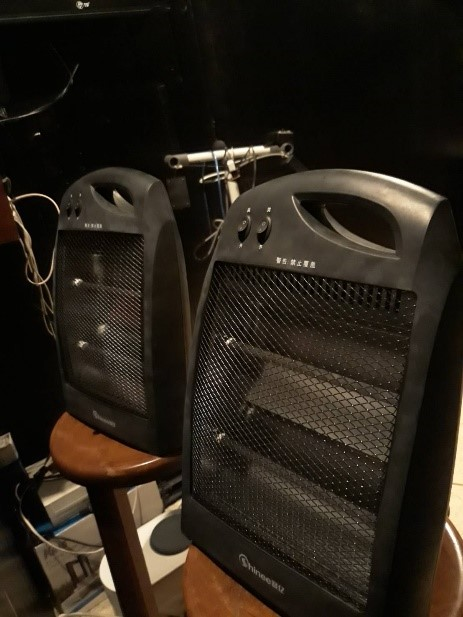
\includegraphics[width=0.5\textwidth]{figures/Heater}
	\caption{Perangkat \textit{Heater}}
	\label{fig:5:Heater}
\end{figure}	

Perangkat AC yang berada di dalam \textit{climate Chamber} DTNTF UGM memiliki daya sebesar 2800W (1 PK). Perangkat AC mampu mengkondisikan lingkungan melalui aliran udara yang keluar. Maka dari itu, Perangkat AC sangatlah berpengaruh terhadap kondisi lingkungan termal di dalam ruangan. Tampak dari wujud perangkat AC dapat dilihat pada Gambar \ref{fig:5:AC}.

Perangkat \textit{heater} yang berada di dalam \textit{climate chamber} memiliki daya sebesar 900W. Terdapat dua buah perangkat \textit{heater} di dalam \textit{climate chamber}. Semakin banyak perangkat heater yang aktif maka akan suhu udara akan menjadi semakin meningkat. Kenaikan rerata suhu udara yaitu sebesar $\pm$1,9$^{\circ}$C untuk setiap perangkat \textit{heater}. Tampak dari wujud perangkat \textit{heater} dapat dilihat pada Gambar \ref{fig:5:Heater}.

Selain faktor dari dalam \textit{climate chamber}, faktor dari luar ruangan \textit{climate chamber} pun secara tidak langsung mempengaruhi kondisi lingkungan termal \textit{climate chamber}. Diantaranya adalah suhu udara luar (\textit{dry bulb temperature}) dan intensitas radiasi matahari. Posisi harian matahari mempengaruhi perubahan nilai suhu udara luar dan intensitas radiasi matahari. Pada siang hari (posisi \textit{altitude} matahari ketika berada tepat diatas \textit{climate chamber}) akan memberikan paparan radiasi matahari yang mengenai selubung bangunan dan menaikkan suhu udara luar. Hal ini menyebabkan suhu di dalam \textit{climate chamber} naik. Kalor yang menembus pada selubung bangunan akan sebanding dengan nilai U-value. Nilai U-Value pada selubung bangunan dapat dilihat pada Tabel \ref{tbl:5:UValue}.

\begin{table}[hbt!]
	\caption{U-Value Selubung \textit{Climate Chamber}}
	\label{tbl:5:UValue}
	\centering
	% use packages: array
	\begin{tabular}{|l|l|}
		\hline
		\textbf{Selubung \textit{climate chamber}} & \textbf{U-Value (W/m$^2$.K)} \\ \hline
		Dinding & 0,707 \\ \hline
		Lantai  & 1,996 \\ \hline
		Atap    & 0,707 \\ \hline
	\end{tabular}
\end{table}

\subsection{Hasil Rancangan Skenario}
Rancangan skenario pada \textit{climate chamber} menghasilkan kombinasi antara set AC dan jumlah \textit{heater} ON. Set AC dikondisikan untuk menyala dari pukul 08:00 s.d. 17:00 dengan rentang nilai 16$^\circ$C - 30$^\circ$C. Set jumlah \textit{heater} ON terbagi menjadi 3 kondisi, yaitu keduanya tidak menyala (berkode 0), salah satu menyala (berkode 1), dan keduanya menyala (berkode 2). Kombinasi tersebut menghasilkan 25 variasi skenario. Untuk variasi suhu luar dan intensitas radiasi matahari, penulis bersama Tanto sepakat untuk menggunakan 4 titik ekstrim bumi terhadap matahari yaitu pada tanggal 21 Maret, 21 Juni, 23 September dan 22 Desember. Kemudian kami melakukan simulasi disetiap titik tersebut dengan kombinasi set \textit{heater} dan set AC seperti pada Gambar \ref{fig:5:HeaterAC}. Sehingga, total skenario yang dihasilkan dari kombinasi tersebut berjumlah 100 skenario.
\begin{figure}[!h]
	\centering
	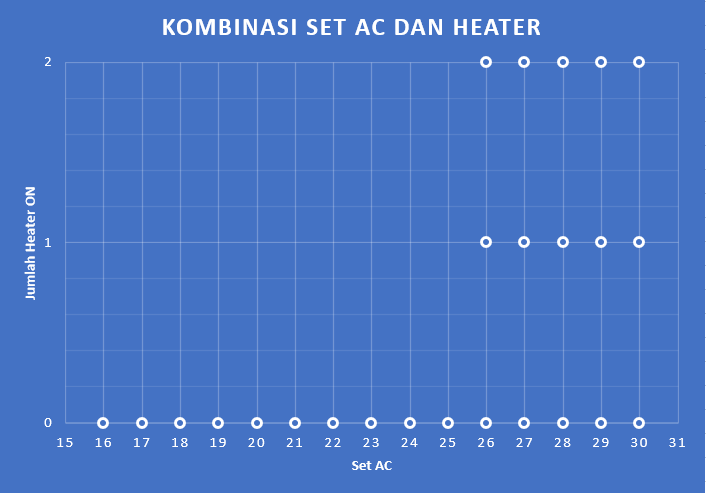
\includegraphics[width=0.8\textwidth]{figures/HeaterAC}
	\caption{Skenario Set Suhu AC dan Jumlah Heater ON}
	\label{fig:5:HeaterAC}
\end{figure}


\subsection{Hasil Simulasi IES-VE}
Pada Gambar \ref{fig:5:HasilIESVE} penulis menunjukan salah satu hasi simulasi untuk skenario SET AC 26$^{\circ}$C dan SET Heater ON 2 buah. Grafik yang ditampilkan terdiri dari 4 parameter yaitu suhu luar (To), intensitas radiasi matahari (Rad), suhu udara ruang (Td), dan kelembapan relatif (RH). 

\begin{figure}[h]
	\centering
	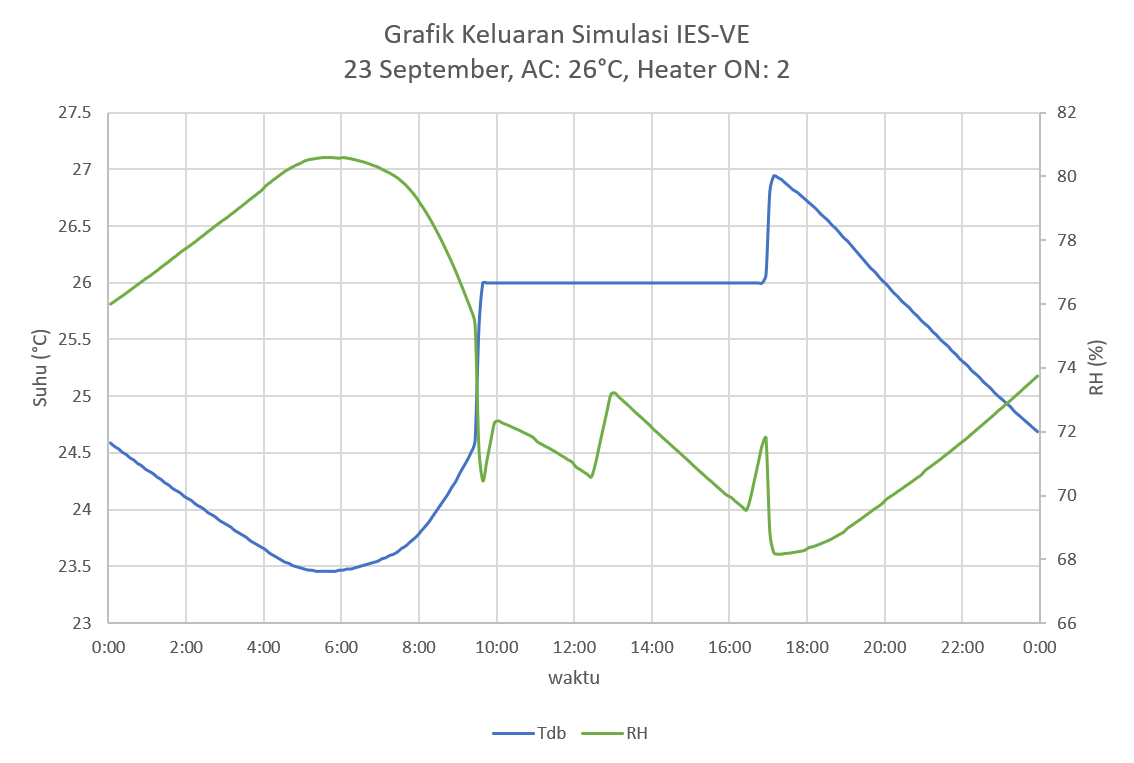
\includegraphics[width=0.8\textwidth]{figures/HasilSimulasiIESVE}
	\caption{Hasil Simulasi IES-VE 23 September, AC 26, Heater ON 2}
	\label{fig:5:HasilIESVE}
\end{figure}

Skenario diatas dilakukan selama 24 jam dengan selang waktu pengambilan data selama 6 menit dimulai dari pukul 00:03 hingga 23:57. Selang waktu tersebut adalah waktu tersingkat yang dapat dilakukan pada \textit{software} IES-VE 2019.

Respon waktu suhu udara terhadap aktivasi AC tidak penulis perhitungkan dikarenakan secara fisis, respons transien termal pada bangunan cukup lama, sehingga para peneliti umumnya hanya fokus untuk meninjau nilai kesalahan keadaan tunak (\textit{steady state error}).

\section{Pemodelan menggunakan NARX}

\noindent \textbf{Penentuan Pembagian Data} 

Dalam menentukan pembagiaan data, penulis melakukan perbandingan dengan beberapa variasi pembagiaan data ke dalam 6 variasi. Kemudian, penulis membandingkan kinerja dari setiap pembagian data dengan menggunakan model JST dengan konfigurasi \textit{hyperparameter} standar dari pustaka \textit{Scikit-Learn}. Pada tabel yang akan penulis sajikan, penulis menulis pembagian data dengan format 'Data Splitting n (x\% y\% z\%)' dimana n = nomor variasi, x = pembagian data pelatihan, y = pembagian data validasi, dan z = pembagian data pengujian. Hasil perbandingan pembagian data dapat dilihat pada Tabel \ref{tbl:5:DataSplitting}
\begin{table}[!h]
	\caption{Daftar variasi pembagian data}
	\label{tbl:5:DataSplitting}
	\centering
	% use packages: array
	\begin{tabular}{|p{6cm}|p{1.5cm}|p{1cm}|p{1.5cm}|p{1cm}|}
		\hline
		\multirow{2}{*}{Pembagian Data } & \multicolumn{2}{|c|}{Training} & \multicolumn{2}{|c|}{Validation} \\
		\cline{2-5}	
		         & EVScore & RMSE & EVScore & RMSE \\
		\hline
		Data Splitting 1 (50\% 25\% 25\%) & 45.58\% & 7.24 & 46.85\% & 7.25 \\
		\hline
		Data Splitting 2 (50\% 30\% 22\%) & 43.56\% & 7.26 & 43.79\% & 7.29 \\
		\hline
		Data Splitting 3 (70\% 15\% 15\%) & 49.21\% & 6.86 & 48.91\% & 6.85 \\
		\hline
		Data Splitting 4 (70\% 20\% 10\%) & 49.29\% & 6.91 & 49.62\% & 6.85 \\
		\hline
		Data Splitting 5 (80\% 10\% 10\%) & 48.69\% & 6.77 & 48.99\% & 6.65 \\
		\hline
		Data Splitting 6 (80\% 15\% 05\%) & 52.09\% & 6.67 & 52.50\% & 6.69 \\
		\hline
	\end{tabular}
\end{table}

Pembagian data terbaik yang penulis gunakan yaitu pembagian data bernama \textit{Data Splitting 6}. Data dibagi menjadi 3 bagian, yakni 80\% data pelatihan, 15\% data validasi, dan 5\% data pengujian. Model JST menggunakan arsitektur \textit{multilayer perceptron} dengan jumlah neuron sebanyak 100 neuron di lapisan tersembunyi 1. \\

\noindent \textbf{Penentuan Nilai Maksimal Iterasi}

Pada \textit{hyperparameter} ini penulis membandingkan dua nilai $max\_iter$, yaitu $max\_iter = 200$ (\textit{default}) dan $max\_iter = 5000$. Perbandingan tersebut disajikan dalam bentuk grafik yang dapat dilihat pada Gambar \ref{fig:5:MaxIter200} dan Gambar \ref{fig:5:MaxIter5000}. \\

\begin{figure}[h]
	\centering
	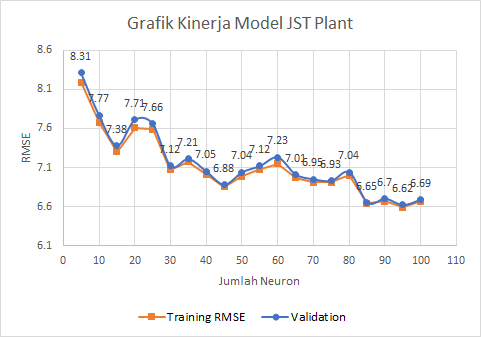
\includegraphics[width=0.8\textwidth]{figures/maxiter200}
	\caption{Grafik kinerja model JST \textit{plant} dengan $max\_iter = 200$}
	\label{fig:5:MaxIter200}
\end{figure}

\begin{figure}[!h]
	\centering
	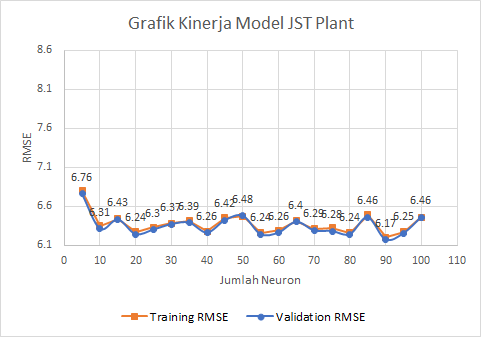
\includegraphics[width=0.8\textwidth]{figures/maxiter5000}
	\caption{Grafik kinerja model JST \textit{plant} dengan $max\_iter = 5000$}
	\label{fig:5:MaxIter5000}
\end{figure}

Berdasarkan kedua grafik tersebut didapatkan hasil bahwa $max\_iter = 5000$ memiliki kinerja lebih baik dibandingkan $max\_iter = 200$ dikarenakan pada $max\_iter = 5000$ model dapat lebih cepat mencapai nilai RMSE yang jauh lebih rendah. \\

\noindent \textbf{Penentuan Jumlah Neuron dan \textit{Hidden Layer}}

Dalam menentukan jumlah neuron dan \textit{hidden layer} yang optimal, penulis melakukan perbandingan \textit{trial and error} pada setiap jumlah neuron. Hasil perbandingan tersebut akan penulis sajikan dalam bentuk grafik-grafik perbandingan. Pertama-tama, penulis mencoba meniliki kinerja model jst dengan jumlah neuron kelipatan 5 dari jumlah neuron bernilai 5 hingga bernilai 100. Kinerja model jst tersebut dapat dilihat pada Gambar \ref{fig:5:Neuron5-100}.
\begin{figure}[!h]
	\centering
	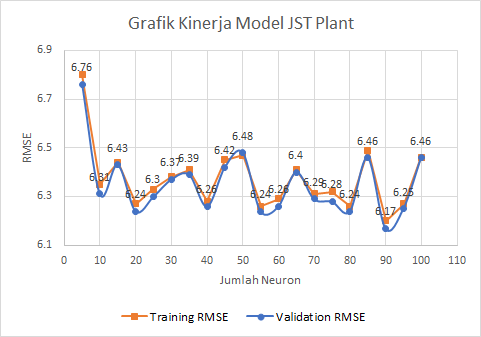
\includegraphics[width=0.9\textwidth]{figures/Neuron5-100}
	\caption{Grafik kinerja model JST \textit{plant} dengan jumlah neuron 5-100}
	\label{fig:5:Neuron5-100}
\end{figure}

Berdasarkan grafik pada Gambar \ref{fig:5:Neuron5-100} didapatkan bahwa nilai RMSE terendah terdapat pada rentang nilai jumah neuron 85-95. Kemudian penulis mencoba membandingan jumlah neuron bernilai 85 hingga 95 dengan rentang perubahan sebesar 1 neuron. Perbandingan tersebut dapat dilihat pada Gambar \ref{fig:5:Neuron85-95}.
\begin{figure}[!h]
	\centering
	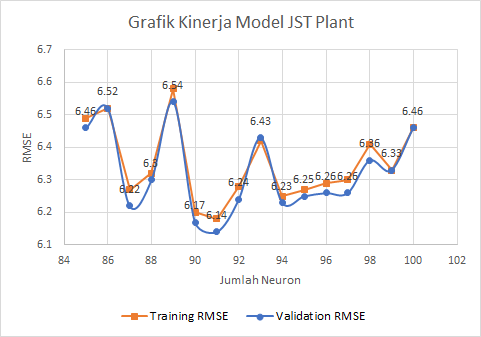
\includegraphics[width=0.9\textwidth]{figures/Neuron85-95}
	\caption{Grafik kinerja model JST \textit{plant} dengan jumlah neuron 85-95}
	\label{fig:5:Neuron85-95}
\end{figure}

Dari grafik pada Gamber \ref{fig:5:Neuron85-95} dapat disimpulkan bahwa jumlah neuron optimal terletak pada nilai 91 neuron, yaitu dengan nilai RMSE = 6,14 pada proses validasi. Nilai ini berlaku untuk model JST dengan arsitektur MLP (\textit{multi-layer perceptron}) dengan \textit{hidden layer} berjumlah 1.

Setelah itu penulis mencoba untuk menilik kinerja model terhadap masing-masing variabel, yaitu terhadap suhu udara (Td) dan kelembapan relatif (RH).
\begin{table}[!h]
	\caption{Tabel Kinerja Model JST Plant 91 Neuron}
	\label{tbl:5:Performance}
	\centering
	% use packages: array
	\begin{tabular}{|p{1.3cm}|p{1.4cm}|p{1cm}|p{0.8cm}|p{0.9cm}|p{0.5cm}|p{1.4cm}|p{1cm}|p{0.8cm}|p{0.9cm}|p{0.5cm}|}
		\hline
		\multirow{2}{*}{Variabel} & \multicolumn{5}{|c|}{Training} & \multicolumn{5}{|c|}{Validation} \\
		\cline{2-11}	
		& EVScore & RMSE & MAE & Mean & Std & EVScore & RMSE & MAE & Mean & Std \\
		\hline
		Td & 82.34\% & 1.05 & 0.74 & -0.13 & 1 & 83.00\% & 1.07 &  0.75 & -0.19 & 1.1 \\
		\hline
		RH & 32.15\% & 8.68 & 7.18 & 0.31 & 8.7 & 34.00\% & 8.62 & 7.20 & 0.19 & 8.6 \\
		\hline
	\end{tabular}
\end{table}

Berdasarkan data pada Tabel \ref{tbl:5:Performance}, dapat dilihat bahwa pada proses validasi (\textit{validation}) masing-masing suhu udara (Td) dan kelembapan relatif (RH) memiliki nilai MAE = 0.75 dan MAE = 7.20. Nilai tersebut merupakan nilai yang dapat diterima oleh tuntutan rancangan pada penelitian ini.\\

\textit{Hyperparameter} yang digunakan pada pembangunan MLP ini dijelaskan pada tabel berikut:

\begin{table}[!h]
	\caption{Tabel Rancangan MLP}
	\label{tbl:5:MLPDesign}
	\centering
	% use packages: array
	\begin{tabular}{|p{5.7cm}|p{5cm}|}
		\hline
		\textbf{Nama Hyperparameter} & \textbf{Nilai Hyperparameter} \\
		\hline
		Jumlah Layar Tersembunyi & 1 \\
		\hline
		Jumlah Neuron pada Layar & [91] \\
		\hline
		Angka Maksimal Iterasi & 5000 \\
		\hline
		Fungsi Aktivasi Layar & ReLU \\
		\hline
		Algoritma Optimisasi (\textit{Solver}) & ADAM \\
		\hline
	\end{tabular}
\end{table}

%\noindent \textbf{Penentuan Algoritma Pembelajaran (\textit{Solver/Optimizer})} \\

%\noindent \textbf{Penentuan \textit{Epoch, Alpha, dan Learning Rate}} \\

\noindent \textbf{{Pembangunan NARX menggunakan MLP yang telah dibuat}} \\

Pembangunan NARX menggunakan pustaka Python bernama \textbf{fireTS}. \textit{Hyperparameter} yang digunakan pada pembangunan NARX ini dijelaskan pada tabel berikut:
\begin{table}[!h]
	\caption{Tabel Rancangan NARX}
	\label{tbl:5:NARXDesign}
	\centering
	% use packages: array
	\begin{tabular}{|p{5.7cm}|p{5cm}|}
		\hline
		\textbf{Nama Hyperparameter} & \textbf{Nilai Hyperparameter} \\
		\hline
		Fungsi estimator & Multilayer Perceptron (MLP) \\
		\hline
		The autoregression order & 1 \\
		\hline
		The exogenous input order & [1,1,1,1] \\
		\hline
		The delay of the exogenous input& [0,0,0,0] \\
		\hline
	\end{tabular}
\end{table}

\subsection{Analisis Kinerja Model}
Persamaan ditulis rata tengah dan nomor persamaan ditulis rata kanan. Nomor persamaan
diurutkan dengan format (nomor\_bab.nomor\_persamaan). Contoh dapat dilihat pada

\section{Pembangunan \textit{Neural Predictive Control}}
Data dibagi menjadi 3 bagian, yakni 70\% data pelatihan, 15\% data validasi, dan 15\% data pengujian. Model JST menggunakan arsitektur \textit{multilayer perceptron} dengan jumlah neuron sebanyak $x_1$ di lapisan tersembunyi 1, $x_2$ di lapisan tersembunyi 2, dan $x_3$ di lapisan tersembunyi 3.

\subsection{Analisis Kinerja Kontroler}
Persamaan ditulis rata tengah dan nomor persamaan ditulis rata kanan. Nomor persamaan
diurutkan dengan format (nomor\_bab.nomor\_persamaan). Contoh dapat dilihat pada Persamaan